\documentclass[11pt]{article}

\usepackage{graphicx}
\usepackage[table,xcdraw]{xcolor}
\usepackage{longtable}

\author{Fanni Dorottya Nagy}
\date{November 22, 2021}
\title{Wedding Registry App Specification}

\begin{document}
    \maketitle

    \section{Description}
    Users (couples or their wedding invitees) can log in and manage their registries and/or contributions to the spouses-to-be.
    Invitees can see all their contributions to different couples in one place and browse registries to buy additional gifts.
    Browsing is made easier by filters, both by present category and price. \\
    Couples can manage their registries (add or remove items) as well as see which items are spoken for already.

    \section{Domain}
    \begin{figure}[h]
        \centering
        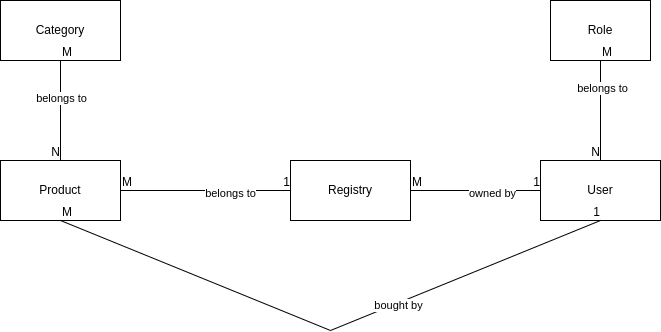
\includegraphics[width=0.7\textwidth]{domain.png}
    \end{figure}
    Note regarding the relationship between registries and products: naturally, there can be identical products that differ only in their ID.
    I.e. semantically the relationship is many-to-many, however, from the point of view of the database these are handled as separate products whose attirbutes just so happens to be the same.

    \section{Use Cases}
    \subsection*{Anonymous}
    \begin{itemize}
        \item log in
    \end{itemize}
    \subsection*{Logged in}
    \begin{itemize}
        \item log out
        \item browse registries
        \item mark product bought/un-bought on others' registries
        \item add/remove items on own registry
        \item view all bought items
    \end{itemize}
    \subsection*{Admin}
    \begin{itemize}
        \item manage users
    \end{itemize}

    \section{API}
    \begin{longtable}{|p{0.2\textwidth}|p{0.8\textwidth}|}
    %\begin{tabular}{|l|l|}
    \hline
    \rowcolor[HTML]{C0C0C0} 
    \multicolumn{1}{|l|}{\cellcolor[HTML]{C0C0C0}\textbf{API}} & GET api/auth/login                                              \\ \hline
    Description                                                & logs in a user               \\ \hline
    Request body                                               & username/password                         \\ \hline
    Response body                                              & -                                              \\ \hline
    Status code                                                & \begin{tabular}[c]{@{}l@{}}200: OK\\ 401: login failed\end{tabular} \\ \hline
    \rowcolor[HTML]{C0C0C0} 
    \multicolumn{1}{|l|}{\cellcolor[HTML]{C0C0C0}\textbf{API}} & GET api/auth/logout                                              \\ \hline
    Description                                                & logs out a user                \\ \hline
    Request body                                               & username/password                         \\ \hline
    Response body                                              & -                                              \\ \hline
    Status code                                                & \begin{tabular}[c]{@{}l@{}}200: OK\\ b\end{tabular} \\ \hline
    \rowcolor[HTML]{C0C0C0} 
    \multicolumn{1}{|l|}{\cellcolor[HTML]{C0C0C0}\textbf{API}} & GET api/categories/{id}                                              \\ \hline
    Description                                                & gets the data of the category with the given id                \\ \hline
    Request body                                               & -                         \\ \hline
    Response body                                              & one category                                              \\ \hline
    Status code                                                & \begin{tabular}[c]{@{}l@{}}200: OK\\ 404: category not found\end{tabular} \\ \hline
    \rowcolor[HTML]{C0C0C0} 
    \multicolumn{1}{|l|}{\cellcolor[HTML]{C0C0C0}\textbf{API}} & POST api/categories                                               \\ \hline
    Description                                                & creates a new category                \\ \hline
    Request body                                               & one category                         \\ \hline
    Response body                                              & one category                                              \\ \hline
    Status code                                                & \begin{tabular}[c]{@{}l@{}}201: category created\\ 400: model validation errors\end{tabular} \\ \hline
    \rowcolor[HTML]{C0C0C0}
    \multicolumn{1}{|l|}{\cellcolor[HTML]{C0C0C0}\textbf{API}} & PUT api/categories/{id}                                              \\ \hline
    Description                                                & updates a category                \\ \hline
    Request body                                               & one category                         \\ \hline
    Response body                                              & -                                              \\ \hline
    Status code                                                & \begin{tabular}[c]{@{}l@{}}204: updated successfully, no content\\ 400: model validation errors\\ 404: category not found\end{tabular} \\ \hline
    \rowcolor[HTML]{C0C0C0}
    \multicolumn{1}{|l|}{\cellcolor[HTML]{C0C0C0}\textbf{API}} & DELETE api/categories/{id}                                              \\ \hline
    Description                                                & deletes a category                \\ \hline
    Request body                                               & -                         \\ \hline
    Response body                                              & -                                              \\ \hline
    Status code                                                & \begin{tabular}[c]{@{}l@{}}204: deleted successfully, no content\\ 404: category not found\end{tabular} \\ \hline
    \rowcolor[HTML]{C0C0C0}
    \multicolumn{1}{|l|}{\cellcolor[HTML]{C0C0C0}\textbf{API}} & GET api/registries?user={userid}                                              \\ \hline
    Description                                                & gets the registry of a specific user                \\ \hline
    Request body                                               & -                         \\ \hline
    Response body                                              & registry of the given user                                              \\ \hline
    Status code                                                & 200: OK \\ \hline
    \rowcolor[HTML]{C0C0C0}
    \multicolumn{1}{|l|}{\cellcolor[HTML]{C0C0C0}\textbf{API}} & GET api/contributions?user={userid}                                              \\ \hline
    Description                                                & get the contributions of a specific user                \\ \hline
    Request body                                               & -                         \\ \hline
    Response body                                              & list of products                                              \\ \hline
    Status code                                                & 200: OK \\ \hline
    \rowcolor[HTML]{C0C0C0}
    \multicolumn{1}{|l|}{\cellcolor[HTML]{C0C0C0}\textbf{API}} & PUT api/contributions                                              \\ \hline
    Description                                                & add a contribution                \\ \hline
    Request body                                               & contribution                         \\ \hline
    Response body                                              & contribution                                              \\ \hline
    Status code                                                & \begin{tabular}[c]{@{}l@{}}201: created\\ 400: model validation errors\end{tabular} \\ \hline
    \rowcolor[HTML]{C0C0C0}
    \multicolumn{1}{|l|}{\cellcolor[HTML]{C0C0C0}\textbf{API}} & DELETE api/contributions/{id}                                            \\ \hline
    Description                                                & delete a contribution                \\ \hline
    Request body                                               & -                         \\ \hline
    Response body                                              & -                                              \\ \hline
    Status code                                                & \begin{tabular}[c]{@{}l@{}}204: deleted successfully, no content\\ 404: contribution not found\end{tabular} \\ \hline
    \rowcolor[HTML]{C0C0C0}
    \multicolumn{1}{|l|}{\cellcolor[HTML]{C0C0C0}\textbf{API}} & GET api/products?registry={registryid}\&minprice={int}\&maxprice={int}\&categories={list of categoryids}                                              \\ \hline
    Description                                                & filter products of a registry based on price and category                \\ \hline
    Request body                                               & -                         \\ \hline
    Response body                                              & list of products that fit the filter criteria                                              \\ \hline
    Status code                                                & 200: OK \\ \hline
    %\end{tabular}
    \end{longtable}
    
    Note: the CRUD operations are the same for registries and products as for categories.
    
    \section{Authentication, Authorization}
    The API can authenticate users.
    Authentication is maintained by JWT tokens.
    Users can belong to roles. \\
    The following roles are specified:
    \begin{itemize}
        \item user
        \item admin
    \end{itemize}
    Anonymous users are not authorized for any action other than logging in. \\
    There are some actions that only admin users can perform.

\end{document}
